\documentclass[11pt,a4paper]{article}
\usepackage{fontspec}
\setmainfont{TeX Gyre Pagella}
\newfontfamily\headfont{Inter}[UprightFont=*-ExtraBold,BoldFont=*-ExtraBold,Extension=.otf,Path=/usr/share/fonts/opentype/inter/]
\usepackage[a4paper,margin=2.3cm]{geometry}
\usepackage{graphicx,booktabs,float,caption,array,xcolor,longtable}
\usepackage{xurl}
\usepackage[hidelinks]{hyperref}
\usepackage{titlesec}
\usepackage[round]{natbib}
\usepackage{setspace}
\setstretch{1.05}
\renewcommand{\topfraction}{0.9}
\renewcommand{\bottomfraction}{0.8}
\renewcommand{\textfraction}{0.1}
\renewcommand{\floatpagefraction}{0.75}
\setlength{\parindent}{0pt}
\setlength{\parskip}{0.55em}
\titleformat{\section}{\headfont\Large}{\thesection}{0.8em}{}
\titleformat{\subsection}{\headfont\large}{\thesubsection}{0.8em}{}
\captionsetup{font=small,labelfont=bf}
\urlstyle{same}
\hypersetup{pdftitle={The Star Fort Belt: How the Bastion Spread Around the World},pdfauthor={Tristan Hotham}}

\begin{document}
\begin{center}
{\Large\bfseries The Star Fort Belt\par}
\vspace{0.4em}
{\large How the bastion spread around the world:\\outlines, dates and sizes of 1,307 star forts from open data\par}
\vspace{1.2em}
{\large Tristan Hotham\par}
\vspace{0.3em}
{\small Independent researcher\\
ORCID: 0000-0003-4931-9349\\
DOI: https://doi.org/10.5281/zenodo.24043680\par}
\vspace{0.8em}
2026
\end{center}

\begin{quote}
\small
\begin{center}\textbf{Abstract}\end{center}
The bastioned fortification, or trace italienne, was devised in Italy around 1500 and built from the Low Countries to Japan over the next three and a half centuries. I assemble an open catalogue of 1,307 star forts in 80 countries: 769 bastioned outlines found by shape in OpenStreetMap, 498 further forts catalogued in Wikidata, and 40 famous forts added from English Wikipedia, after setting aside 253 outlines that are probably towered walls of other traditions and 560 Bavarian listed earthworks of uncertain form. Only 251 forts (19\%) can be dated, 84 of them by hand. 89\% of the forts lie in Europe, in a belt along the war zones from the Low Countries to the Baltic. The earliest dated works are Italian, but the bastion did not spread outwards from Italy: a country's distance from Florence barely predicts the date of its first dated fort (Spearman's $\rho$ = 0.15, 49 countries), and the median first date is 1623 for countries beyond Europe against 1626 within it, because Portuguese and Spanish ships carried it to India, Africa and the Caribbean in the 1530s and 1540s. The traced outlines are small (median 1.9 ha, about 228 m across) and most often have four points (42\%); size does not change with date. 59\% of the catalogued forts still have an outline that a shape test recognises.

\textbf{Keywords:} star fort; bastion; trace italienne; military architecture; diffusion; OpenStreetMap; Wikidata; historical GIS
\end{quote}

\section{Introduction}
Between the 1490s and the 1530s Italian engineers answered the siege gun with a new kind of wall: low, thick and angled, with projecting bastions placed so that every face could be swept by fire from a neighbour. The resulting star-shaped trace, the trace italienne, became the standard fortification of early modern Europe and of the European empires, and historians have tied it to the growth of armies, the cost of war and the reach of European power overseas \citep{parker,duffy}. Its spread is usually told through famous examples: Michele Sanmicheli's Verona, the ideal city of Palmanova, the Dutch fortress belt, Vauban's France, and the colonial forts from Goa to Havana.

This study asks what an open, systematic catalogue can add. Where are the star forts that survive or are recorded? When were they built, and how far can the dates be trusted? Did the design spread outward from Italy, or did it jump? How large were they, how many points did they have, and how many survive on the ground? The work accompanies an interactive map drawn on The Inked World basemap \citep{inkmap} at \url{https://maps.tristanhotham.com/star-forts/}, with a decade slider and every fort's sources.

\section{Data}
\textbf{Outlines.} The forts come from The Inked World \citep{inkmap}, which extracted from OpenStreetMap \citep{osm} every way and relation tagged as a fort or fortification, every town wall and every moat, joined broken walls and moats into rings, and kept the rings that look like a bastioned trace (Section~\ref{sec:methods}). This gives 1,022 outlines. It also added 1,061 forts from Wikidata \citep{wikidata} that belong to the classes star fort (Q12797), sconce (Q91203, Q6653030) or polygonal fort (Q92080) but have no traced outline.

\textbf{Dates and names.} For every Wikidata item I queried, with QLever, the inception (P571) with its precision, start time (P580), official opening (P1619), dissolution or demolition (P576), classes and architect, and the full list of items under star fort and fortified town (Q677678) with coordinates and dates. From the OpenStreetMap extract I read the name, \texttt{wikidata} and \texttt{start\_date} tags of every element lying on each outline. Finally, I dated 84 important forts by hand from their English Wikipedia articles \citep{wikipedia}, recording the year the bastioned works were begun, the builder, and whether the works survive (Appendix, Table~\ref{tab:hand}). Countries and town names come from Natural Earth \citep{ne}.

\section{Methods}\label{sec:methods}
\subsection{Finding a star}
A ring counts as bastioned when, simplified to 4 m, it has a perimeter between 250 m and 20 km, fills between 45\% and 93\% of its convex hull, and has at least four salient corners: convex corners sharper than 100 degrees that lie further from the centre than their neighbours, at distances from the centre that vary by no more than a quarter, with at least as many re-entrant corners between them. Rings named or catalogued as star forts or sconces need only three. I keep the number of salients as the fort's ``points''. Because rings joined from broken walls and moats are made with round buffers that soften the bastion points, the maps and Figure~\ref{fig:strip} draw each fort from its own wall, rampart and moat pieces at full detail instead; the rings are used only to find and measure the forts. Its area, perimeter and largest diameter are measured on a local plane.

\subsection{Cleaning the catalogue}
Catalogue points lying on an outline were merged into it (3), and Wikidata fortified towns lying inside an outline gave it their name and identifier. Outlines with no name in either source (603) are named after the nearest Natural Earth town. Two groups are kept in the data but left out of every count: 560 entries from the Bavarian monument list that Wikidata labels as sconces, whose form and age are unknown; and 253 outlines in countries where the shape test mostly finds fortifications of other traditions (the towered walls of Chinese and Korean towns, Mughal and Rajput forts, North African medinas, Persian and Central Asian forts), unless dated by hand as a European work, together with a few known false matches such as Maginot Line blocks. The result is 1,307 forts: 769 with an outline, 498 Wikidata points and 40 points added from Wikipedia.

\subsection{Choosing a date}
Each fort takes the first available of: the hand date; Wikidata's start time or opening; Wikidata's inception if precise to the year or decade; the OpenStreetMap start date. Dates before 1450 are the medieval origin of a site rather than its bastions and are set aside (10 forts), as are inceptions of monasteries and decade-precision inceptions before 1550. A country's first fort is its earliest dated fort in the data, and its distance is the great-circle distance from Florence to that fort. Diffusion is tested with Spearman's rank correlation between first year and distance.

\section{Results}
\subsection{The belt}
1,165 of the 1,307 forts (89\%) are in Europe (Figure~\ref{fig:belt}). They form a belt along the early modern war zones: the Low Countries and northern France, the Rhine, the Alps and the Po valley, the Venetian and Habsburg frontiers, the border between Spain and Portugal, and the Baltic. The densest one-degree cell, in the Netherlands around the Rhine and Maas delta, holds 39 forts. Malta has the highest density by far, then the Netherlands (24.9 per 10,000 km$^2$) and Belgium (9.1). Sweden has the most forts of any country (297), but 295 of them are small sconces catalogued from the national heritage register, a reminder that the catalogue measures recording as well as building (Table~\ref{tab:countries}).

\begin{figure}[tbp]\centering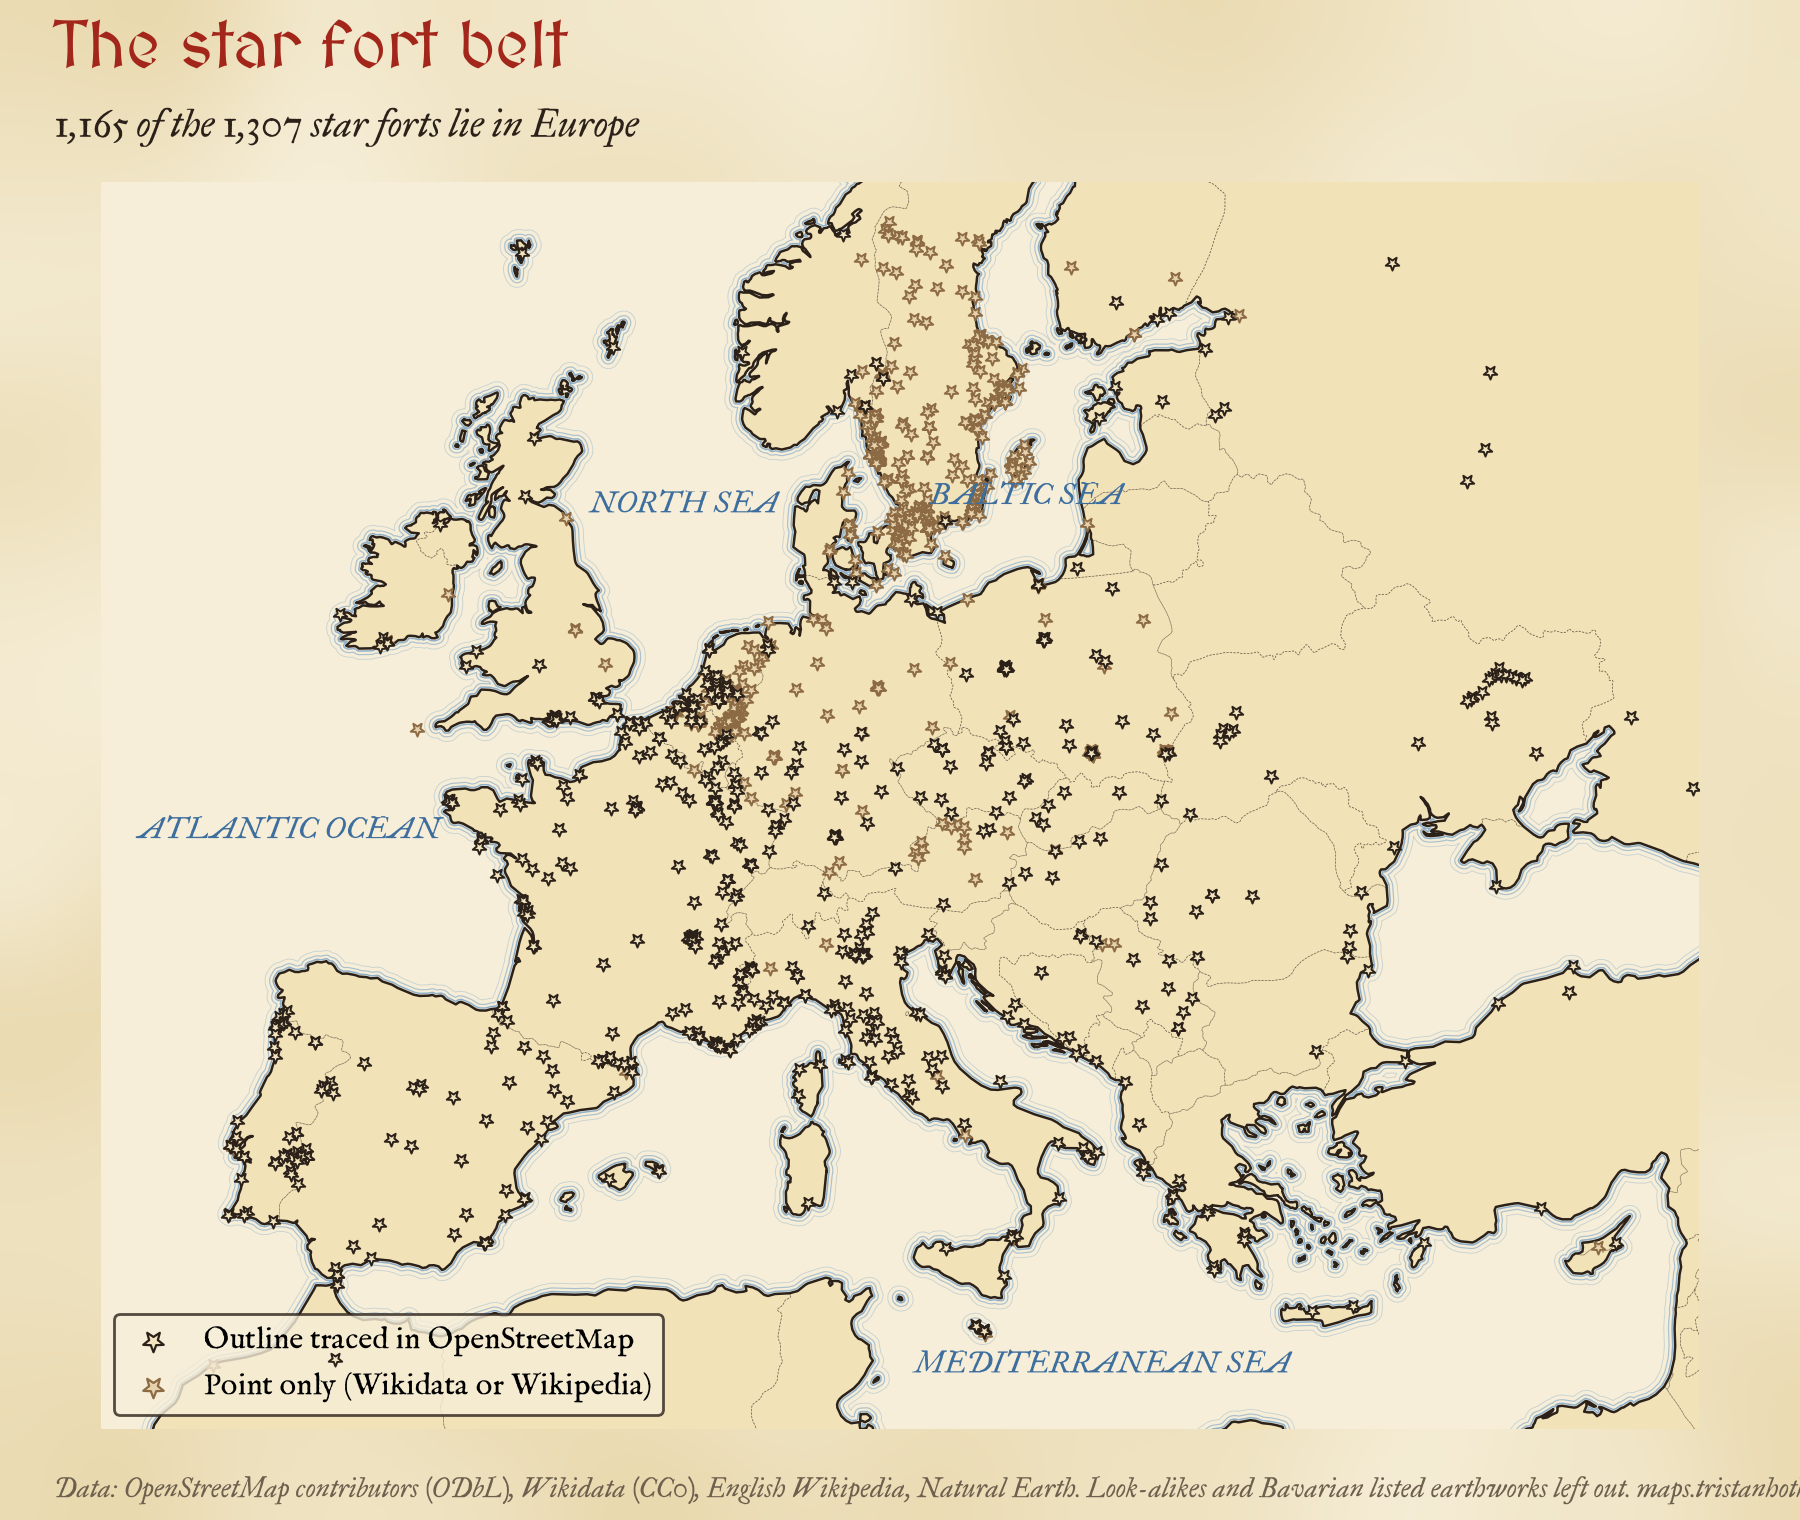
\includegraphics[width=\textwidth]{f_belt.png}
\caption{Star forts in Europe and around the Mediterranean, by whether an outline is traced in OpenStreetMap.}\label{fig:belt}\end{figure}

\begin{table}[tbp]\centering\small\caption{The twelve countries with most star forts: all forts, those with a traced outline, and those with a date.}\label{tab:countries}\begin{tabular}{lrrr}\toprule Country & Forts & Outlines & Dated\\\midrule
Sweden & 297 & 2 & 7\\
France & 170 & 169 & 30\\
Netherlands & 93 & 27 & 12\\
Italy & 88 & 83 & 29\\
Poland & 66 & 34 & 14\\
Germany & 60 & 23 & 14\\
Spain & 55 & 54 & 3\\
Portugal & 47 & 46 & 11\\
United States of America & 39 & 37 & 18\\
Ukraine & 30 & 30 & 3\\
Belgium & 28 & 13 & 7\\
United Kingdom & 26 & 21 & 12\\
\bottomrule\end{tabular}\end{table}

\subsection{Dates}
251 forts (19\%) have a date: 84 by hand, 127 from Wikidata and 40 from OpenStreetMap. Without the hand dates only 13\% would be dated. Of the dated forts, 20\% were begun before 1600, 26\% in the 1600s, 21\% in the 1700s and 34\% from 1800, when polygonal forts with low bastions or caponiers continued the type (Figure~\ref{fig:decades}). The dated forts peak in the 1590s, the 1670s and the 1870s; the dated forts beyond Europe peak in the 1750s and 1760s, the decades of the Seven Years' War.

\begin{figure}[tbp]\centering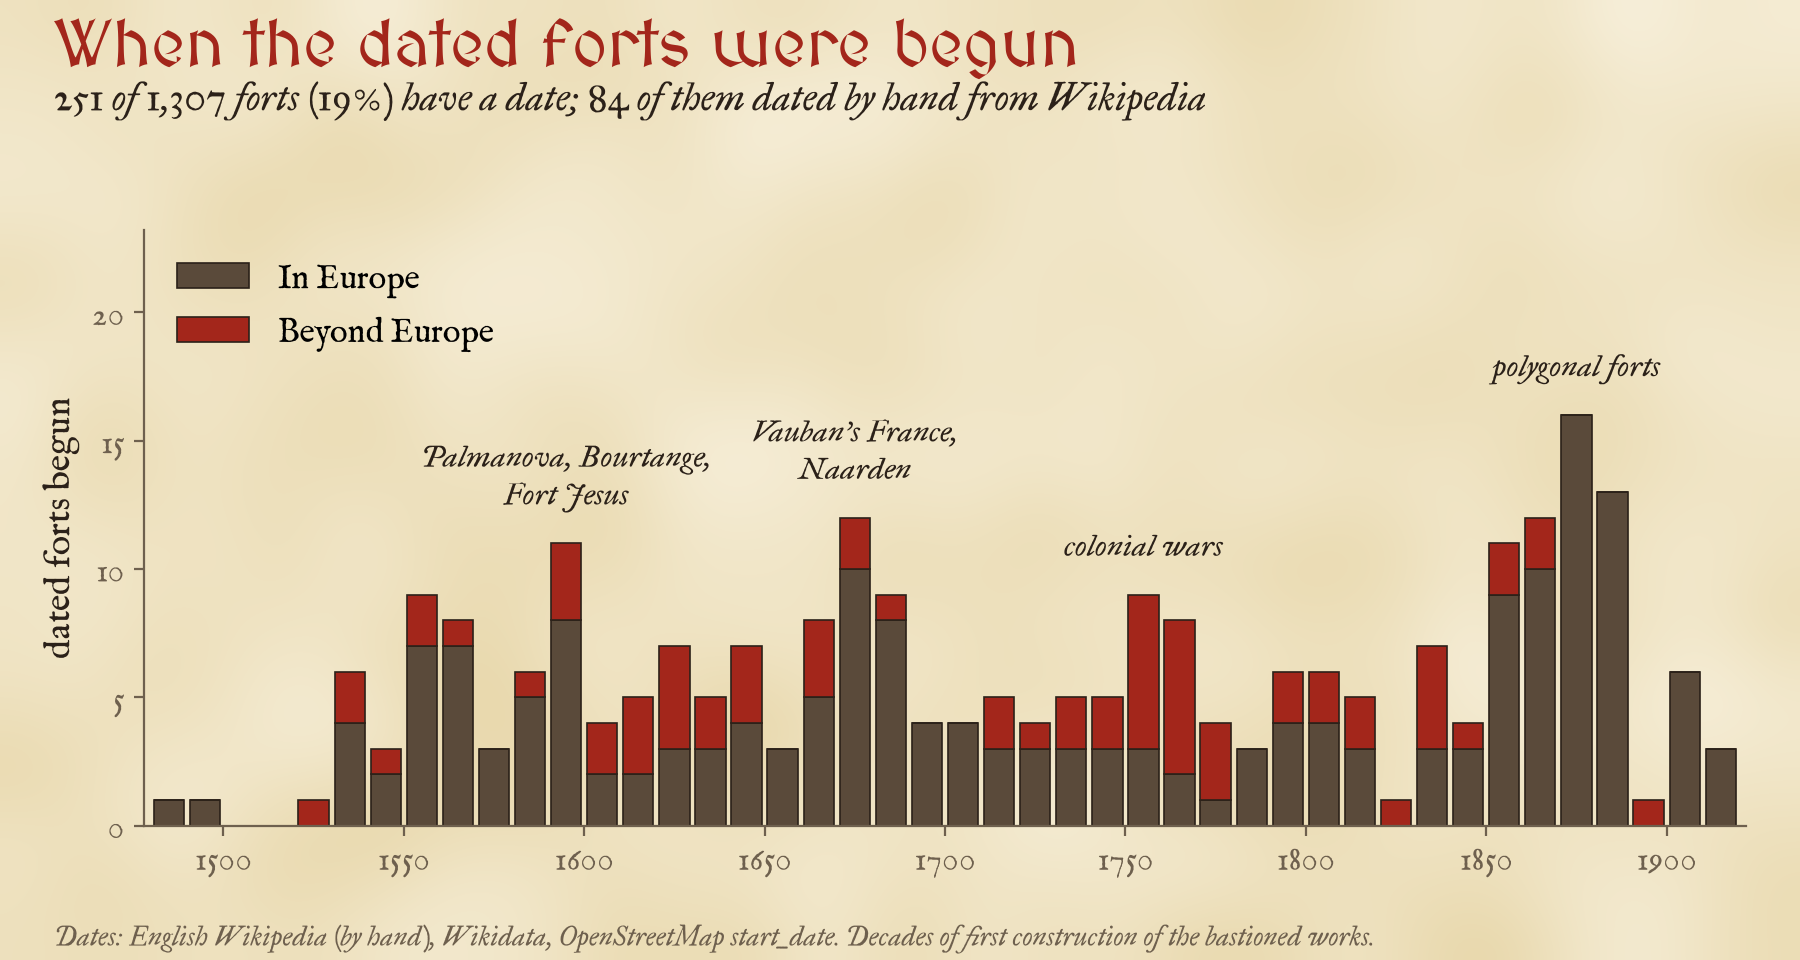
\includegraphics[width=\textwidth]{f_decades.png}
\caption{Dated star forts by decade begun, in Europe and beyond.}\label{fig:decades}\end{figure}

\subsection{Diffusion}
The earliest dated works in the data are Italian, Cassero della Fortezza (1488) and the Fortezza da Basso in Florence (1534). Table~\ref{tab:regions} gives the earliest dated fort in each region. The design reached the Low Countries, the German lands, England and Sweden in the 1540s and 1550s, but it reached India, Morocco and Puerto Rico in the same decades (Figure~\ref{fig:first}). Across the 49 countries with a dated fort, distance from Florence barely predicts the date of the first one ($\rho$ = 0.15, $p$ = 0.32; within Europe $\rho$ = 0.29 across 27 countries, $p$ = 0.15). Countries beyond Europe have a median first date of 1623, against 1626 in Europe (Figure~\ref{fig:distance}). The bastion travelled by sea, with the Portuguese and Spanish empires, as fast as it travelled by land.

\begin{table}[tbp]\centering\footnotesize\caption{Regions: forts, dated forts and their share (\%), the earliest dated fort in the data and the median year of the dated forts.}\label{tab:regions}\begin{tabular}{p{3.6cm}rrrp{4.2cm}rr}\toprule Region & Forts & Dated & \% & Earliest dated & Year & Median\\\midrule
Italy and Malta & 97 & 34 & 35 & Cassero della Fortezza & 1488 & 1725\\
Iberia & 102 & 14 & 14 & Fort of São Julião da Barra & 1553 & 1623\\
France & 171 & 30 & 18 & Fort-Carré & 1553 & 1723\\
Low Countries & 125 & 19 & 15 & Fort Rammekens & 1547 & 1673\\
German lands and Central Europe & 176 & 32 & 18 & Citadel of Jülich & 1548 & 1806\\
Scandinavia and the Baltic & 344 & 21 & 6 & Landskrona Citadel & 1559 & 1677\\
British Isles & 34 & 14 & 41 & Berwick-upon-Tweed walls & 1558 & 1858\\
Eastern Europe, Balkans and Turkey & 116 & 17 & 15 & Venetian walls of Nicosia & 1567 & 1734\\
Africa & 15 & 4 & 27 & Mazagan & 1541 & 1575\\
Americas & 87 & 42 & 48 & Castillo San Felipe del Morro & 1539 & 1760\\
Asia and Oceania & 40 & 24 & 60 & Fort Kastela & 1522 & 1644\\
\bottomrule\end{tabular}\end{table}

\begin{figure}[tbp]\centering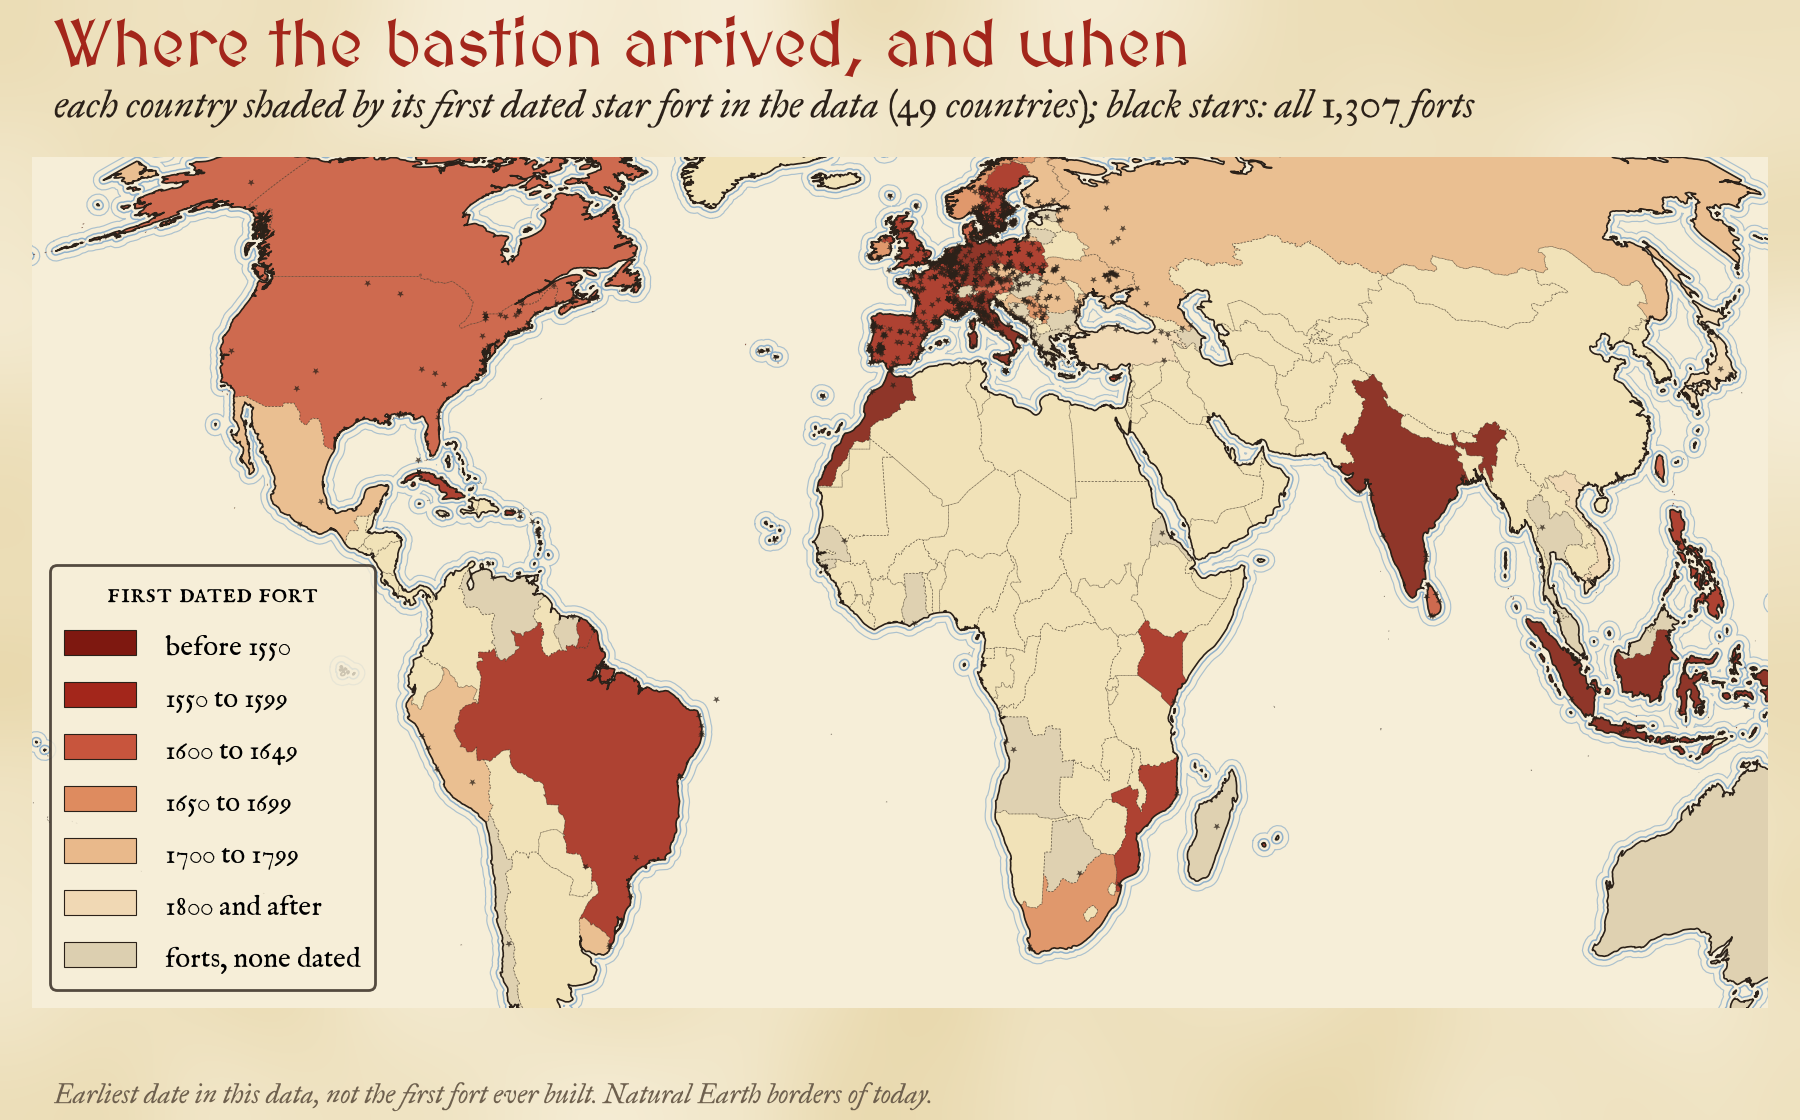
\includegraphics[width=\textwidth]{f_first.png}
\caption{Countries by the period of their first dated star fort in the data. Brown-grey: forts present, none dated.}\label{fig:first}\end{figure}

\begin{figure}[tbp]\centering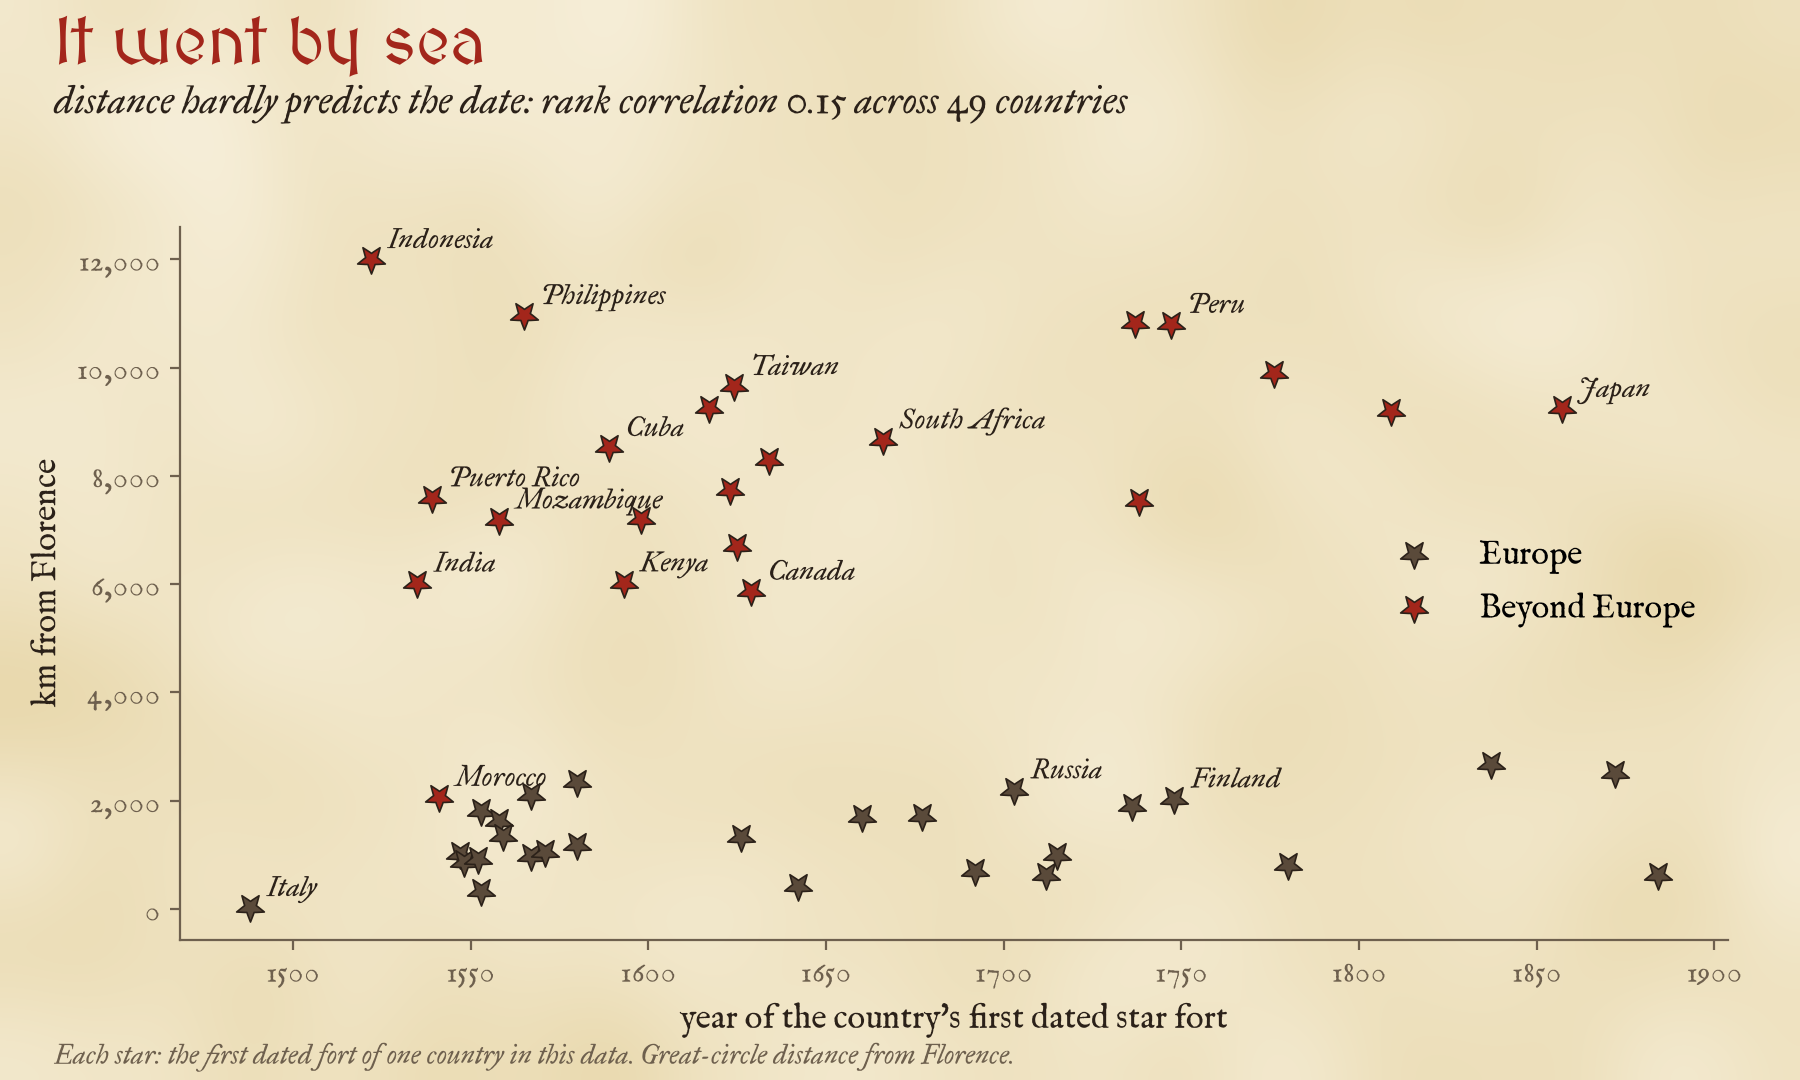
\includegraphics[width=\textwidth]{f_distance.png}
\caption{Year of each country's first dated star fort against its distance from Florence.}\label{fig:distance}\end{figure}

\subsection{The colonial chain}
33 of the hand-dated forts are outside Europe (Figure~\ref{fig:chain}). Their order follows the empires: Portugal from Diu (1535), Spain from San Juan (1539), the Dutch East India Company from Banda Neira (1611), the English East India Company from Madras (1640), France on Cape Breton Island (1720), Denmark on St Croix (1738), the United States at Baltimore (1798) and, last, the Tokugawa shogunate at Hakodate (1857). The selection is mine and favours famous forts, so the chain is an illustration rather than a measurement.

\begin{figure}[tbp]\centering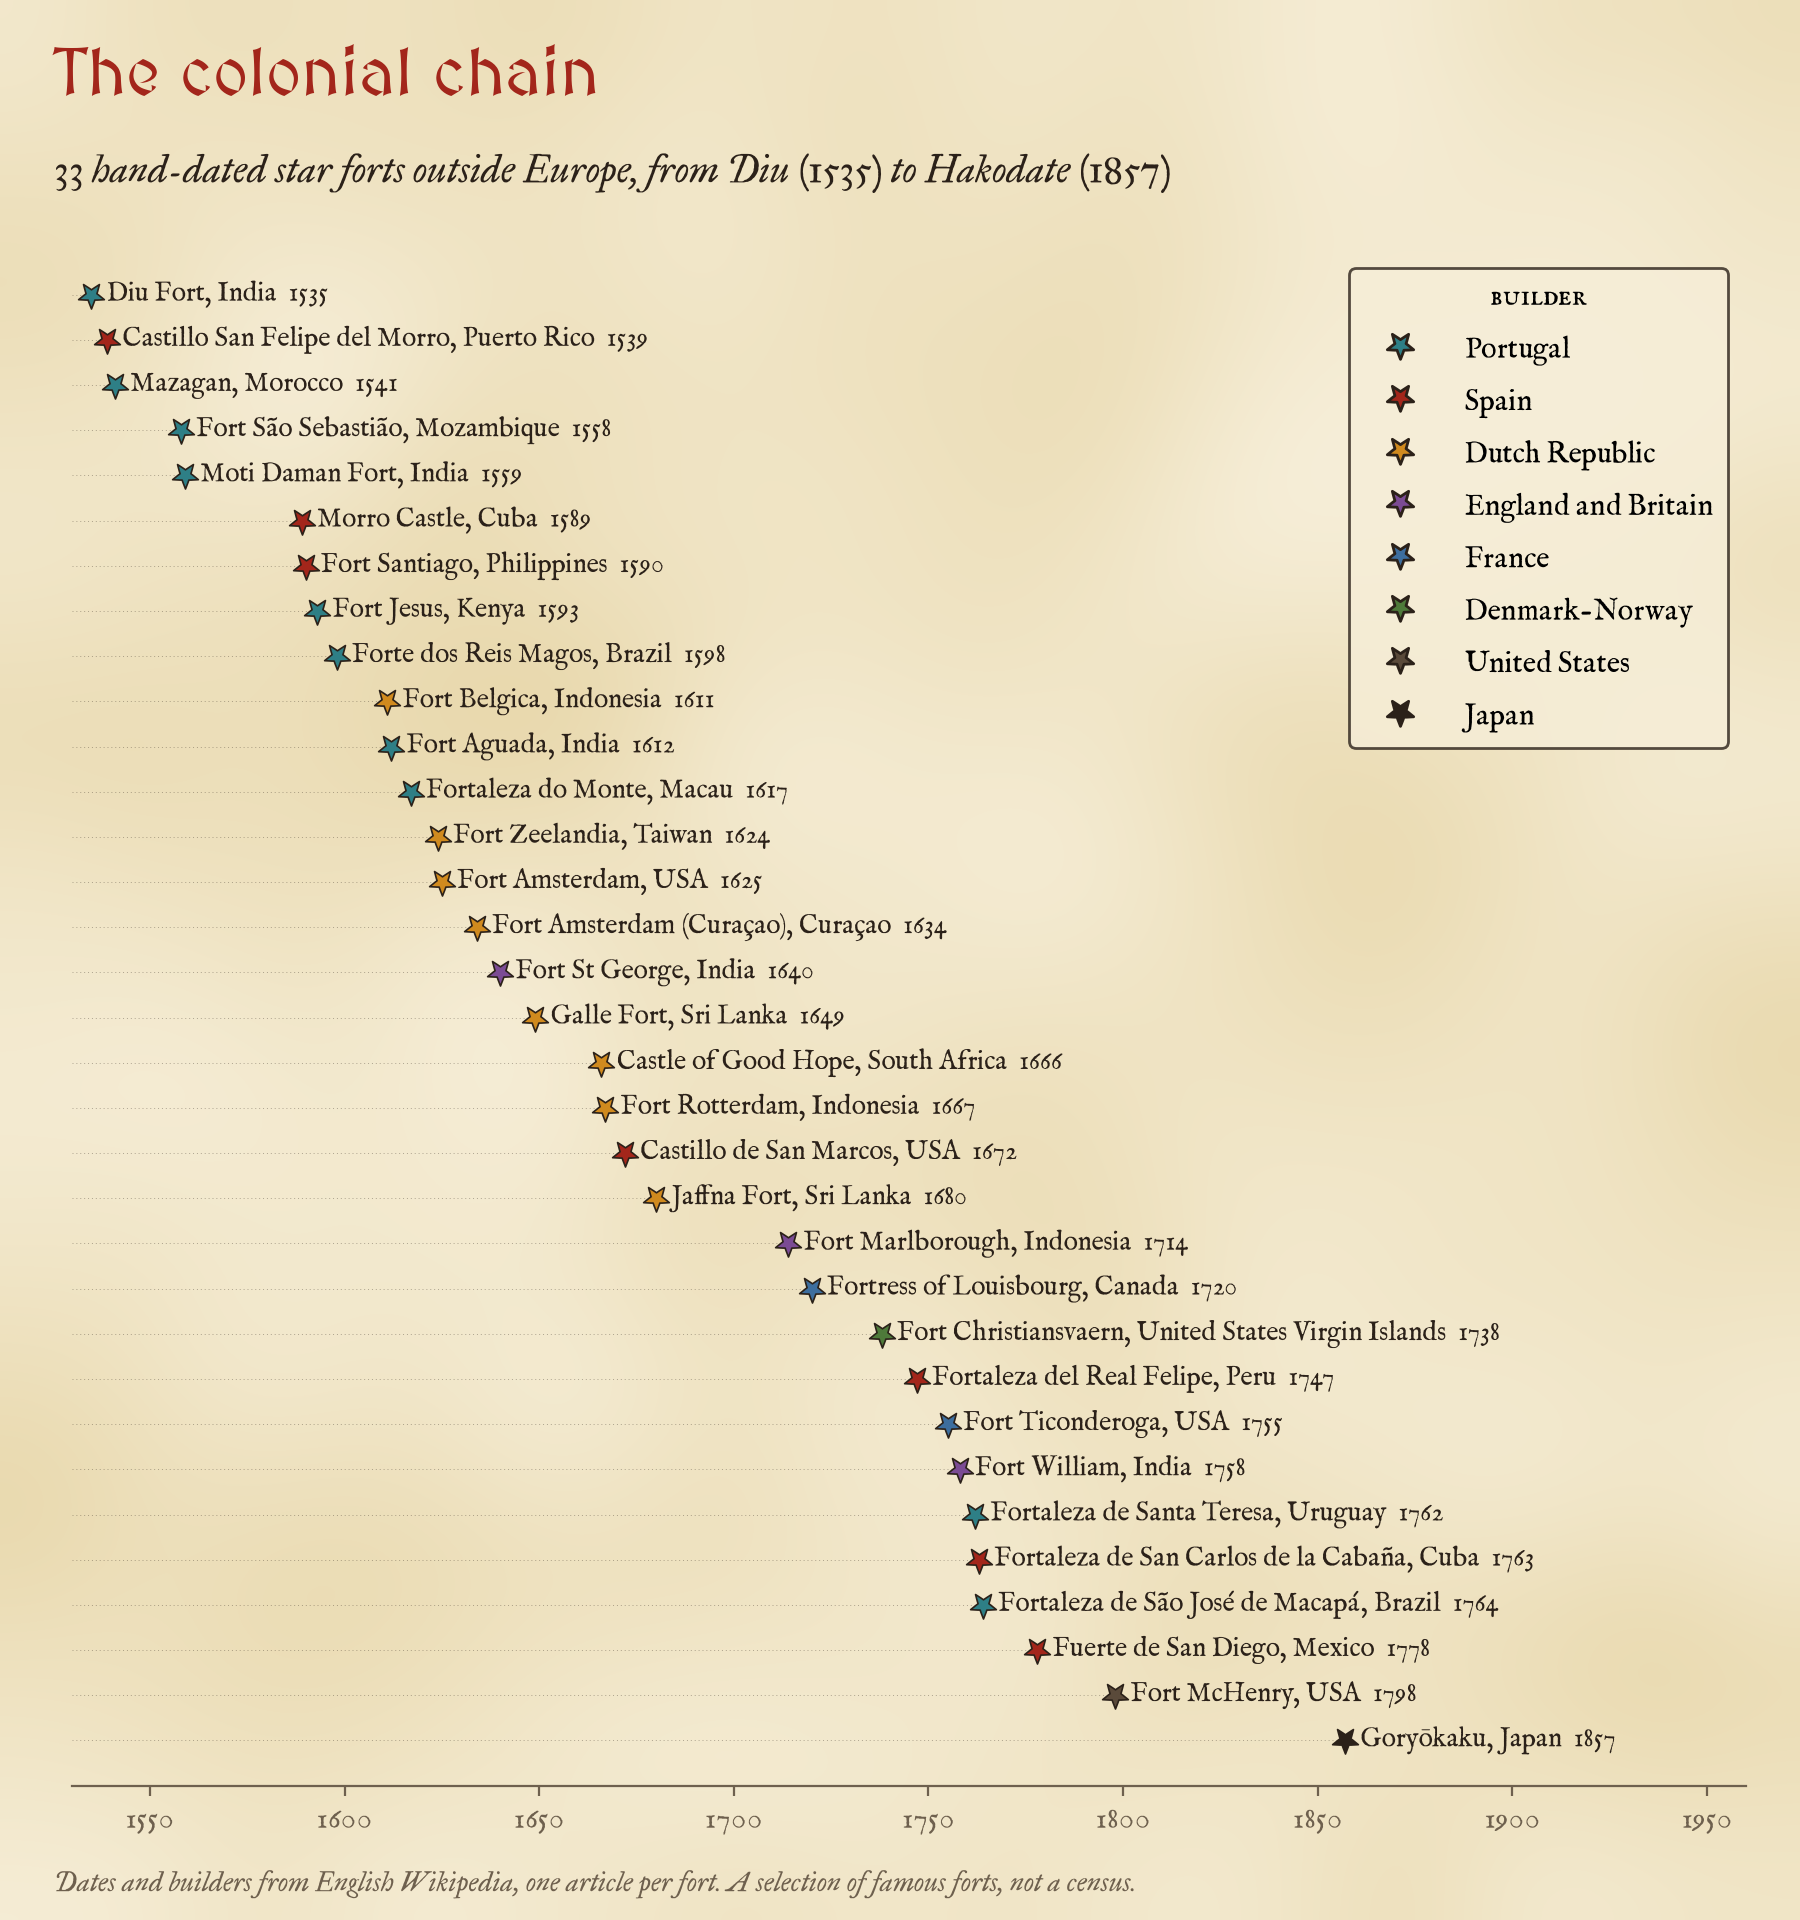
\includegraphics[width=\textwidth]{f_chain.png}
\caption{Hand-dated star forts outside Europe, in order of the year begun, coloured by builder.}\label{fig:chain}\end{figure}

\subsection{Size and form}
The 769 outlines have a median area of 1.9 ha (interquartile range 0.7 to 4.0 ha) and a median diameter of 228 m; 53\% enclose less than 2 ha, 89 more than 10 ha and 9 more than 50 ha (Figure~\ref{fig:sizes}). Four points is the commonest form (320 outlines, 42\%), and 72\% have four, five or six. The largest outlines are fortress towns and nineteenth-century ring fortresses (Table~\ref{tab:largest}). Among the dated outlines, size does not change with date ($\rho$ = -0.02, 172 forts): the median is 1.4 ha before 1600, 2.6 ha in the 1600s, 1.6 ha in the 1700s and 2.4 ha from 1800. Figure~\ref{fig:strip} draws twelve famous outlines at one scale.

\begin{figure}[tbp]\centering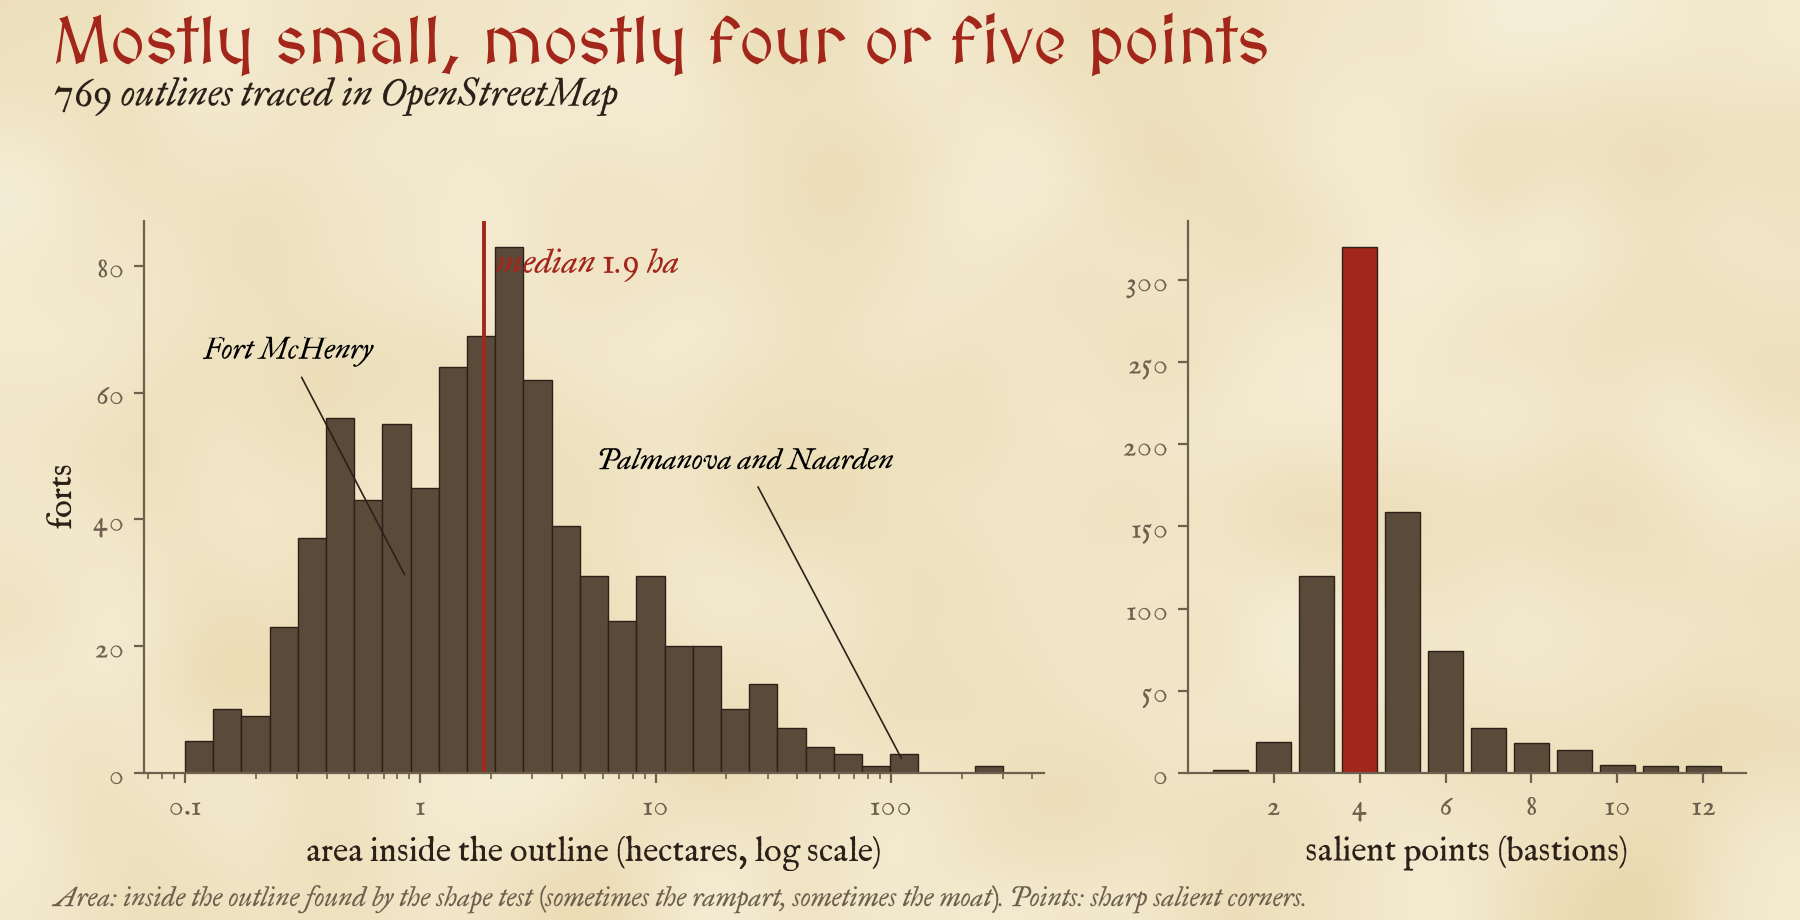
\includegraphics[width=\textwidth]{f_sizes.png}
\caption{Area inside the traced outlines (log scale) and number of salient points.}\label{fig:sizes}\end{figure}

\begin{figure}[tbp]\centering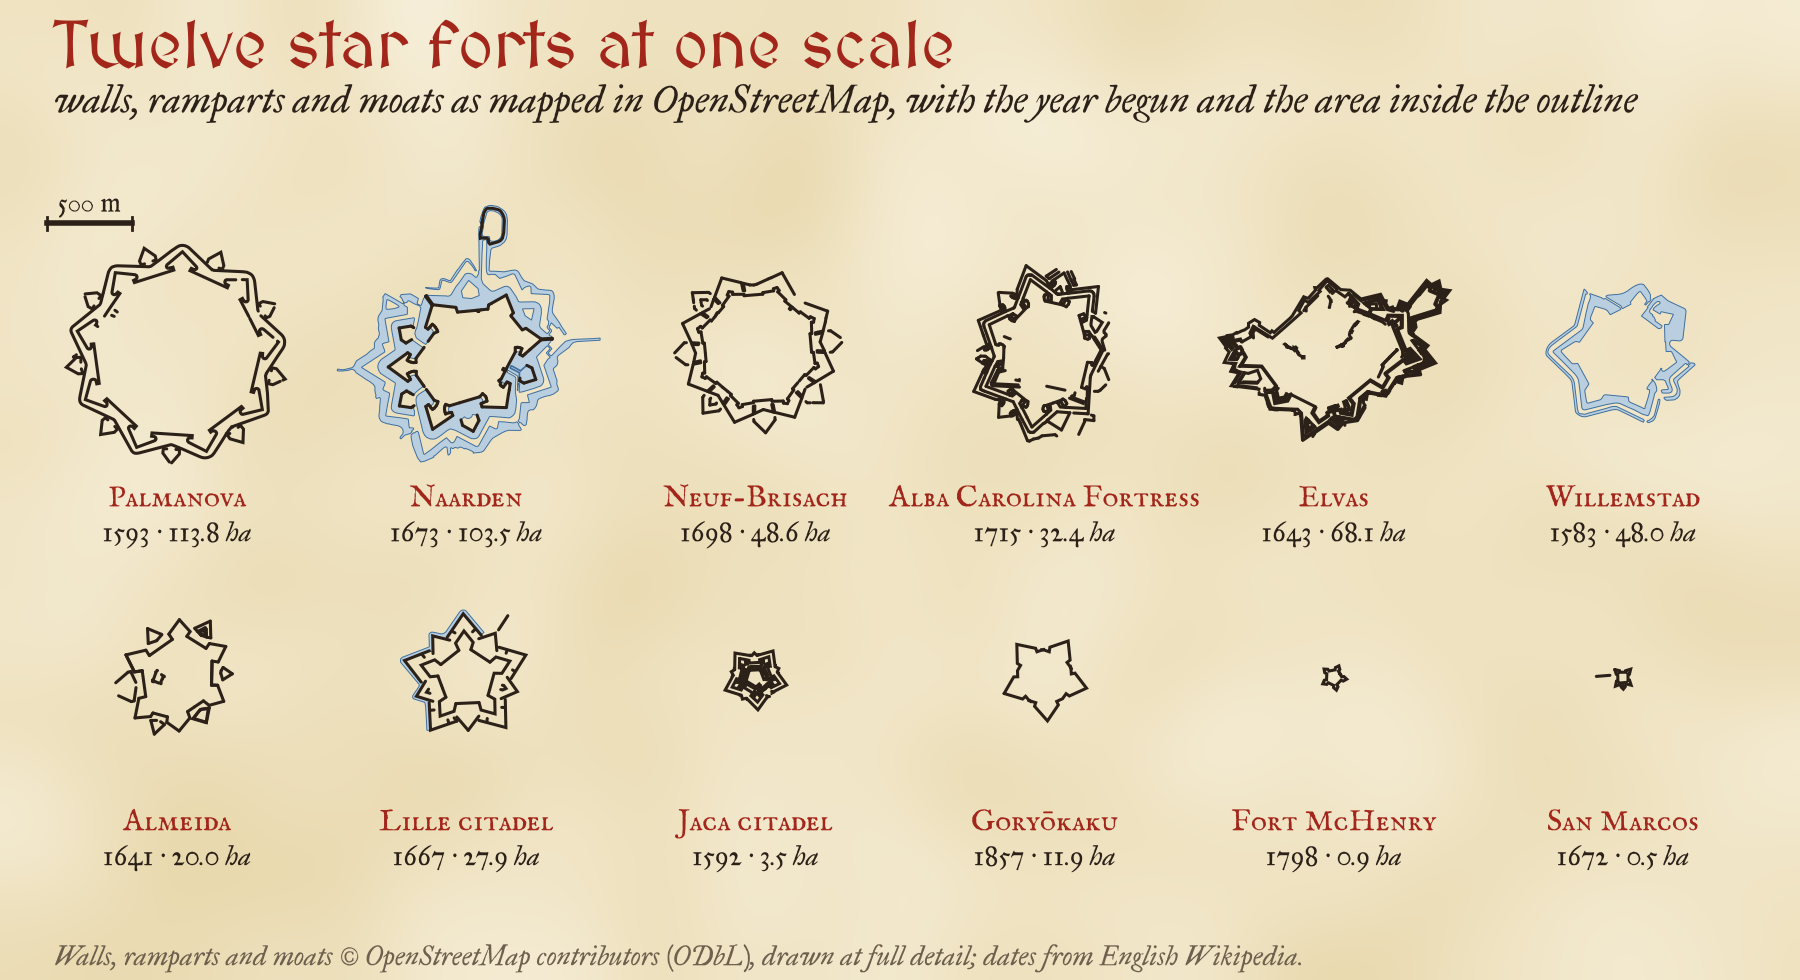
\includegraphics[width=\textwidth]{f_strip.png}
\caption{Twelve star forts at one scale, from their OpenStreetMap outlines.}\label{fig:strip}\end{figure}

\begin{table}[tbp]\centering\small\caption{The twelve largest traced outlines (unnamed ones carry the name of the nearest town).}\label{tab:largest}\begin{tabular}{llrrr}\toprule Fort & Country & Area (ha) & Points & Begun\\\midrule
Twierdza Modlin & Poland & 228.8 & 5 & 1806\\
Star fort near Pisa & Italy & 130.7 & 4 & \\
Palmanova & Italy & 113.8 & 8 & 1593\\
Naarden & Netherlands & 103.5 & 5 & 1673\\
Fort Monroe National Monument & United States of America & 80.0 & 4 & 1834\\
Elvas & Portugal & 68.1 & 17 & 1643\\
Valletta & Malta & 66.5 & 12 & 1566\\
Famagusta within the walls & Cyprus & 59.3 & 7 & \\
Festung Mont Royal & Germany & 51.0 & 3 & \\
Star fort at Rodos & Greece & 49.5 & 7 & \\
Neuf-Brisach & France & 48.6 & 8 & 1698\\
Willemstad & Netherlands & 48.0 & 4 & 1583\\
\bottomrule\end{tabular}\end{table}

\subsection{Survival}
59\% of the forts have an outline that the shape test still recognises; the share is 56\% in Europe and 82\% beyond it, where the catalogue is made mostly of large, well-known forts. Of the 84 hand-dated forts, 46\% have a traced outline; 5 are known to have been largely demolished (the citadels of Antwerp and Turin, Saarlouis, Fort Amsterdam on Manhattan and Louisbourg, the last partly rebuilt). A missing outline is not proof of loss: it can also mean a fort mapped in pieces, or one too eroded or too irregular to pass the test.

\section{Limitations}
First, the catalogue is what has been mapped and catalogued. OpenStreetMap is richest in Europe; Wikidata's sconces come in bulk from a few national registers (Sweden, Bavaria, the Netherlands); and countless earthwork sconces and siege works left no trace. Second, the shape test both misses forts (irregular traces, forts mapped as fragments, coastal forts that use the shore) and finds look-alikes; I removed the look-alikes by country, a blunt rule that also removes some genuine forts. Third, only a fifth of the forts are dated, and the hand-dated ones are a selection of famous forts, so the timeline and the colonial chain lean to the well known. Fourth, inception dates can refer to a site's first fortification rather than its bastions. Fifth, the area of a fort is the area inside the line the shape test found, sometimes the inner rampart and sometimes the outer edge of a moat. Sixth, the country of each fort is its modern country.

\section{Conclusion}
Seen as data, the star fort is a European belt with a long colonial tail. The dated record, thin as it is, shows the design leaving Italy by two routes at once: overland to the war zones of northern Europe, and by sea to the Portuguese and Spanish ports of three continents, where it arrived as early as it did in much of Europe. Most forts were small and square or pentagonal; a few were towns. Two in five no longer show their star to a shape test.

\section*{Data and code availability}
The interactive map is at \url{https://maps.tristanhotham.com/star-forts/}. Data and code are at \url{https://github.com/Tristan-Hotham/star-forts} and archived with this paper at https://doi.org/10.5281/zenodo.24043680. Tables derived from OpenStreetMap (the outlines and the fort table) are released under the Open Database License 1.0; Wikidata content is CC0; text and figures are CC BY 4.0 and code MIT.

\section*{AI statement}
I wrote the text, with drafting and editing assistance from Claude (Anthropic), which also helped prepare the analysis code. I reviewed and checked all text and results.

\begin{thebibliography}{9}
\bibitem[Duffy(1979)]{duffy} Duffy, C. (1979) \textit{Siege Warfare: the Fortress in the Early Modern World, 1494 to 1660}. London: Routledge.
\bibitem[Hotham(2026)]{inkmap} Hotham, T. (2026) The Inked World: a zoomable hand-inked style world map from open data. \url{https://maps.tristanhotham.com/ink-map/}
\bibitem[Natural Earth(2026)]{ne} Natural Earth (2026) Admin 0 countries, land and populated places. Public domain. \url{https://www.naturalearthdata.com/}
\bibitem[OpenStreetMap(2026)]{osm} OpenStreetMap contributors (2026) OpenStreetMap, via the Overpass API. ODbL 1.0. \url{https://www.openstreetmap.org/}
\bibitem[Parker(1988)]{parker} Parker, G. (1988) \textit{The Military Revolution: Military Innovation and the Rise of the West, 1500 to 1800}. Cambridge: Cambridge University Press.
\bibitem[Wikidata(2026)]{wikidata} Wikidata contributors (2026) Wikidata, queried with QLever. CC0. \url{https://www.wikidata.org/}
\bibitem[Wikipedia(2026)]{wikipedia} Wikipedia contributors (2026) English Wikipedia articles on the forts listed in Table~\ref{tab:hand}. CC BY-SA 4.0. \url{https://en.wikipedia.org/}
\end{thebibliography}

\clearpage
\appendix
\section{The hand-dated forts}
{\footnotesize\setlength{\tabcolsep}{4pt}\begin{longtable}{p{4.6cm}p{3.2cm}rp{3.2cm}ll}\caption{The 84 forts dated by hand from English Wikipedia: year the bastioned works were begun, builder, whether an outline is traced, and fate. Article links are in data/hand\_dates.csv.}\label{tab:hand}\\\toprule Fort & Country & Begun & Builder & Outline & Today\\\midrule\endfirsthead\toprule Fort & Country & Begun & Builder & Outline & Today\\\midrule\endhead
Forte Spagnolo & Italy & 1534 & Spain & no & survives\\
Fortezza da Basso & Italy & 1534 & Florence & yes & survives\\
Diu Fort & India & 1535 & Portugal & no & survives\\
Castel Sant'Elmo & Italy & 1537 & Spain & no & survives\\
Castillo San Felipe del Morro & Puerto Rico & 1539 & Spain & no & survives\\
Mazagan & Morocco & 1541 & Portugal & no & survives\\
Citadel of Jülich & Germany & 1548 & Jülich-Cleves-Berg & no & survives\\
Fort St Elmo & Malta & 1552 & Knights of St John & yes & survives\\
Fort of São Julião da Barra & Portugal & 1553 & Portugal & no & survives\\
Rocroi & France & 1555 & France & no & survives\\
Berwick-upon-Tweed walls & United Kingdom & 1558 & England & no & survives\\
Fort São Sebastião & Mozambique & 1558 & Portugal & yes & survives\\
Moti Daman Fort & India & 1559 & Portugal & no & survives\\
Spandau Citadel & Germany & 1559 & Brandenburg & no & survives\\
Fortezza Medicea di Siena & Italy & 1561 & Florence & yes & survives\\
Venetian walls of Bergamo & Italy & 1561 & Venice & no & survives\\
Citadel of Turin & Italy & 1564 & Savoy & no & vanished\\
Valletta & Malta & 1566 & Knights of St John & yes & survives\\
Citadel of Antwerp & Belgium & 1567 & Spain & no & vanished\\
Venetian walls of Nicosia & Cyprus & 1567 & Venice & no & survives\\
Citadel of Pamplona & Spain & 1571 & Spain & yes & survives\\
Zamość & Poland & 1580 & Poland-Lithuania & no & survives\\
Willemstad & Netherlands & 1583 & Dutch Republic & yes & survives\\
Wülzburg & Germany & 1588 & Brandenburg-Ansbach & no & survives\\
Morro Castle & Cuba & 1589 & Spain & yes & survives\\
Fort Santiago & Philippines & 1590 & Spain & yes & survives\\
Citadel of Jaca & Spain & 1592 & Spain & yes & survives\\
Bourtange & Netherlands & 1593 & Dutch Republic & yes & survives\\
Fort Jesus & Kenya & 1593 & Portugal & no & survives\\
Palmanova & Italy & 1593 & Venice & yes & survives\\
Star Castle & United Kingdom & 1593 & England & no & survives\\
Forte dos Reis Magos & Brazil & 1598 & Portugal & no & survives\\
Citadel of Gozo & Malta & 1599 & Knights of St John & yes & survives\\
Fort Belgica & Indonesia & 1611 & Dutch Republic & yes & survives\\
Fort Aguada & India & 1612 & Portugal & no & survives\\
Fortaleza do Monte & Macau & 1617 & Portugal & yes & survives\\
Glückstadt & Germany & 1617 & Denmark-Norway & no & survives\\
Fort Zeelandia & Taiwan & 1624 & Dutch Republic & no & survives\\
Fort Amsterdam & United States of America & 1625 & Dutch Republic & no & vanished\\
Kastellet & Denmark & 1626 & Denmark-Norway & no & survives\\
Fort Amsterdam (Curaçao) & Curaçao & 1634 & Dutch Republic & no & survives\\
Fort St George & India & 1640 & England & no & survives\\
Almeida & Portugal & 1641 & Portugal & yes & survives\\
Forte de Santa Luzia & Portugal & 1641 & Portugal & yes & survives\\
Elvas & Portugal & 1643 & Portugal & yes & survives\\
Galle Fort & Sri Lanka & 1649 & Dutch Republic & yes & survives\\
Fredericia & Denmark & 1650 & Denmark-Norway & no & survives\\
Fort Saint-Nicolas & France & 1660 & France & yes & survives\\
Fredrikstad Old Town & Norway & 1663 & Denmark-Norway & no & survives\\
Petersberg Citadel & Germany & 1665 & Electorate of Mainz & no & survives\\
Castle of Good Hope & South Africa & 1666 & Dutch Republic & no & survives\\
Citadel of Lille & France & 1667 & France & yes & survives\\
Fort Rotterdam & Indonesia & 1667 & Dutch Republic & yes & survives\\
Tilbury Fort & United Kingdom & 1670 & England & yes & survives\\
Castillo de San Marcos & United States of America & 1672 & Spain & yes & survives\\
Naarden & Netherlands & 1673 & Dutch Republic & yes & survives\\
Charles Fort & Ireland & 1677 & England & yes & survives\\
Mont-Louis & France & 1679 & France & yes & survives\\
Jaffna Fort & Sri Lanka & 1680 & Dutch Republic & yes & survives\\
Saarlouis & Germany & 1680 & France & no & vanished\\
Citadel of Saint-Martin-de-Ré & France & 1681 & France & yes & survives\\
Citadel of Blaye & France & 1685 & France & yes & survives\\
Petrovaradin Fortress & Serbia & 1692 & Habsburg Monarchy & no & survives\\
Neuf-Brisach & France & 1698 & France & yes & survives\\
Peter and Paul Fortress & Russia & 1703 & Russia & no & survives\\
Fort Marlborough & Indonesia & 1714 & Great Britain & no & survives\\
Alba Carolina Fortress & Romania & 1715 & Habsburg Monarchy & yes & survives\\
Fortress of Louisbourg & Canada & 1720 & France & yes & vanished\\
Fort Christiansvaern & United States Virgin Islands & 1738 & Denmark-Norway & no & survives\\
Fortaleza del Real Felipe & Peru & 1747 & Spain & no & survives\\
Fort George & United Kingdom & 1748 & Great Britain & yes & survives\\
Suomenlinna & Finland & 1748 & Sweden & no & survives\\
Castle of Sant Ferran & Spain & 1753 & Spain & no & survives\\
Fort Ticonderoga & United States of America & 1755 & France & no & survives\\
Fort William & India & 1758 & Great Britain & no & survives\\
Fortaleza de Santa Teresa & Uruguay & 1762 & Portugal & yes & survives\\
Fortaleza de San Carlos de la Cabaña & Cuba & 1763 & Spain & yes & survives\\
Forte de Nossa Senhora da Graça & Portugal & 1763 & Portugal & yes & survives\\
Fortaleza de São José de Macapá & Brazil & 1764 & Portugal & no & survives\\
Fuerte de San Diego & Mexico & 1778 & Spain & no & survives\\
Josefov & Czech Republic & 1780 & Habsburg Monarchy & no & survives\\
Terezín & Czech Republic & 1780 & Habsburg Monarchy & no & survives\\
Fort McHenry & United States of America & 1798 & United States & yes & survives\\
Goryōkaku & Japan & 1857 & Japan & yes & survives\\
\bottomrule\end{longtable}}
\end{document}
